% this TeX file provides an awesome example of how TeX will make super 
% awesome tables, at the cost of your of what happens when you try to make a
% table that is very complicated.
% Originally turned in for Dr. Nico's Security Class
\documentclass[11pt]{article}


% Use wide margins, but not quite so wide as fullpage.sty
\marginparwidth 0.5in 
\oddsidemargin 0.25in 
\evensidemargin 0.25in 
\marginparsep 0.25in
\topmargin 0.25in 
\textwidth 6in \textheight 8 in
% That's about enough definitions

% multirow allows you to combine rows in columns
%\usepackage{multirow}
% tabularx allows manual tweaking of column width
\usepackage{tabularx}
% longtable does better format for tables that span pages
\usepackage{longtable}

\usepackage{graphicx} % allows inclusion of graphics

\usepackage{cite}


\begin{document}
% this is an alternate method of creating a title
%\hfill\vbox{\hbox{Gius, Mark}
%       \hbox{Cpe 456, Section 01}  
%       \hbox{Lab 1}    
%       \hbox{\today}}\par
%
%\bigskip
%\centerline{\Large\bf Lab 1: Security Audit}\par
%\bigskip
\author{Zander Mausolff}
\title{Assessment of TDKENO/MOOSE Coupling for Simulating Transients with Thermal Feedback}
\maketitle

\section{Introduction}
The accurate simulation of transient experiments typically requires thermal feedback to account for a variety of phenomenon such as Doppler broadening. To improve the transient analysis code TDKENO an investigation has begun into the best methods for incorporating thermal feedback. A large motivation is to improve the capabilities of modeling the TREAT reactor at the INL. TDKENO has proven capable of calculating values in agreement with TREAT experimental results.  The caveat is the reliance on feedback provided through empirical TREAT data, thus the approach is not robust.
The rapid transient conditions induced in TREAT experiments deposits rapidly deposits heat into the core.  Unlike commercial LWRs and BWRs there is no water moderator/coolant to complicate the heat-up model.  To better simulate these experiments it is desirable to utilize a simple heat-up model coupled to a neutronics solver. The primary objective is to enable the updating of cross sections at the new temperatures to account for Doppler Broadening, which is thought to influence the TREAT experiments greatly.  

\section{Overview of TDKENO}
To provide context for the coupling implementation a brief description of the Improved Quasi Static (IQS) method within TDKENO is given.  TDKENO is a transient analysis tool that solves the time dependent Boltzmann transport equation with the explicit representation of delayed neutrons. It does so with the IQS Method, which allows the flux profile to vary in time.  The main difference between the original Quasi-Static and IQS is the time derivative in IQS is handled explicitly with a backwards Euler approximation \cite{goluoglu2001time}. 

The basic assumption in IQS is that the total neutron flux can be factored into a shape and amplitude function \cite{Gehin}.  
\begin{equation}
\label{factor}
    \phi(\bar{r},\bar{\Omega}',E,t) = A(t)\Psi(\bar{r},\bar{\Omega}',E,t)
\end{equation}
In Equation \ref{factor} $A$ is the amplitude function, and $\Psi$ is the shape function.
The amplitude function captures the time dependence and takes on physical significance by being cast into the form of the point kinetics equations as follows:

\begin{equation}
    \label{eq:pt_kin}
    \frac{dA(t)}{dt} = \frac{\rho(t)-\bar{\beta}(t)}{\Lambda(t)} A(t) + \sum_{j=1}^{6} \lambda_jC_j(t) + \bar{Q}(t)
\end{equation}

where $P(t)$ is the amplitude function, $\rho$ is reactivity, $\bar{\beta}$ is the effective delayed neutron fraction, $\Lambda$ is the generation time, $\lambda_j$ is the decay constant per neutron group $j$, $C_j$ is the density of delayed neutron precursors for group j, and $\bar{Q}$ is a source.

 Reactivity, generation time, etc. in TDKENO are found from their inner product definitions using a linearly interpolated flux shape. Exact expressions can be found in reference \cite{Bentley}.  Alternatively, these values may be computed during the Monte Carlo random walk but requires significant neutron histories to achieve reasonable statistics \cite{Waddell}.  The shape function varies slowly in time and solves a modified version of the steady state transport equation.  This allows the flux profile to vary in time.  The main modification here is an adjustment to the total cross section \cite{goluoglu2001time, Gehin}.  At present TDKENO calculations are limited to multi-group cross sections, tpyically 238.  In TDKENO the shape equation is solved via Monte Carlo, but in principle the shape equation may be solved with deterministic methods.  Reference \cite{Shayesteh} provides an excellent rationale for implementing Monte Carlo techniques for the flux shape calculation.  A complete derivation of the IQS method used in TDKENO can be found in reference \cite{Bentley}. 
 
 The implementation in TDKENO is hybrid in nature because it relies on a Monte Carlo calculation for the flux shape and a deterministic one for the point kinetics.  The Monte Carlo calculation coming from a modified version of KENO (either V.a or VI).  One can think of TDKENO as a solver of the point kinetics equations that drives the time dependence and calls upon KENO to provide the flux shape at desired times. 
 \begin{figure}[h]
     \centering
     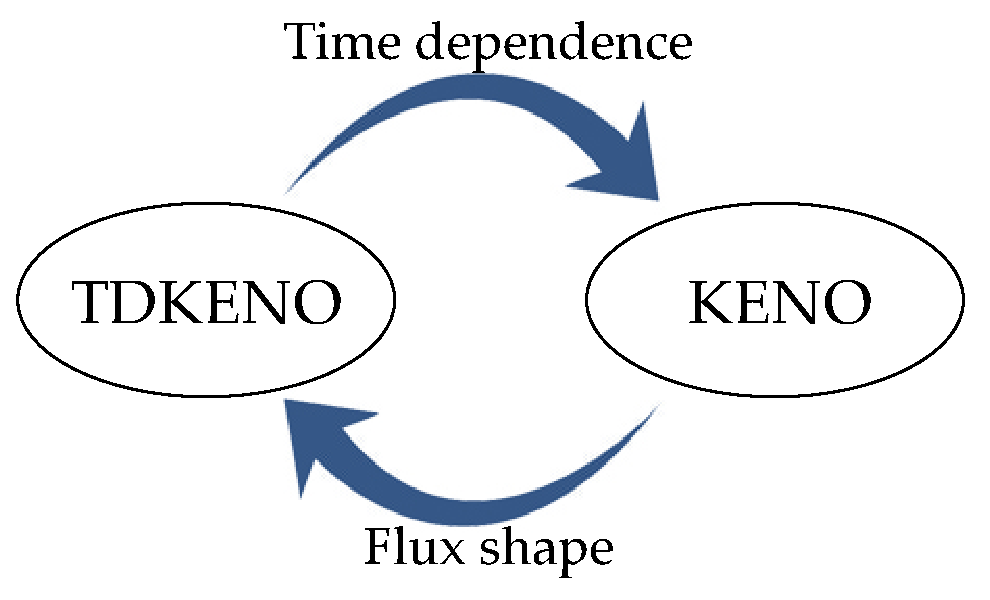
\includegraphics[width=8cm]{figures/tdkeno_flow.pdf}
     \caption{Simplified model of TDKENO calculation}
     \label{fig:simpletdk}
 \end{figure}

Applying the factorization in equation \ref{factor} to the three-dimensional time-dependent transport equation with the explicit representation of delayed neutrons results in a set of coupled equations.  Equations for the flux shape, amplitude, and delayed neutron precursors are solved on several time scales through an iterative process. The relative sizes are shown in Figure \ref{fig:time_scale}. 

\begin{figure}[h]
    \centering
    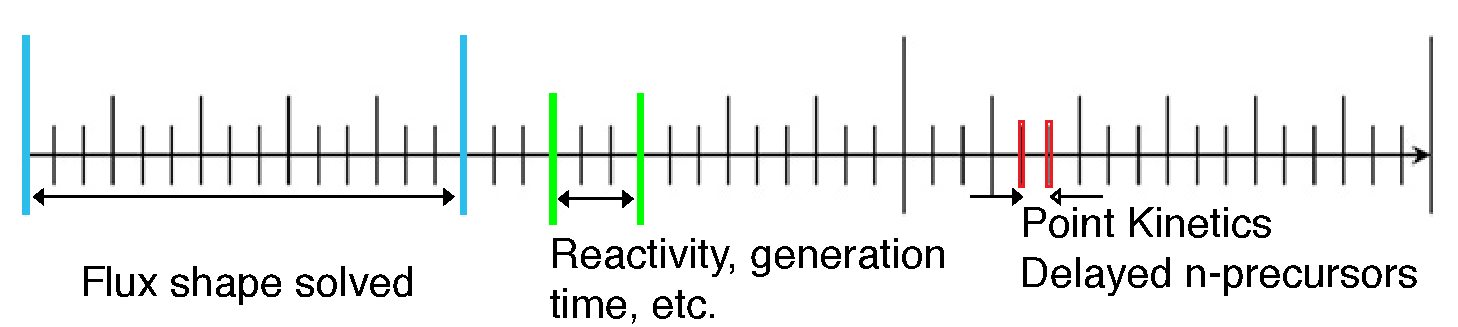
\includegraphics[width=10cm]{figures/time_scale.pdf}
    \caption{Time scale variation for IQS.}
    \label{fig:time_scale}
\end{figure}

The advantage of varying these time scales is less computational time compared to direct integration.  This comes from the flux shape being solved on a large time step. It is only done when the spatial distribution of neutrons changes significantly.  In between flux shapes, equation \ref{eq:pt_kin} is solved to capture the time dependent behavior.  Other IQS implementations are possible, such as the "Predictor Corrector" method.  Here one solves for the total flux and uses the shape in conjunction with the amplitude to correct the total flux \cite{Dulla}.  

 In its current formulation, TDKENO does not do this but rather lets the user define when a flux shape should be calculated.  This gives flexibility and may allow for computational savings as transients experience a rapid change in neutron distribution that is generally known about \emph{a posteriori} and can be accounted for by the user. 

\section{Current Status of TDKENO}
Feedback is incorporated into TDKENO on a problem-specific basis.  For example an empirical model from historical data is implemented for TREAT simulations. This model calculates a correction factor for the reactivity from the yield as follows:
\begin{equation}
    \rho_{fb}(t) = \sum_{i = 0}^{3}a_i Y^i (t)
\end{equation}
where $\rho_{fb}(t)$ is the feedback reactivity, $Y^i (t)$ is the total yield in the core at time $t$, and $a_i$ is the empirical coefficient for a third order polynomial.
  This provides reasonable answers but previous simulations show significant deviations from experiment in calculating the peak power.  For the transient experiments simulated it over calculates the peak power significantly.  However, the yield calculated agrees well with experiment.
Quenching coefficients and several problem specific feedback methods were included in the past.  A simple adiabatic model was put in place for a benchmark problem in \cite{Bentley}.  There is an obvious need for a more generalized feedback method and one that captures the physics better.  The IQS methodology complicates this with several time scales and complex iterative scheme.  

\section{Method for Incorporating Thermal Feedback}

For TREAT experiments and most transients, the thermal effect to be resolved is the Doppler broadening of cross sections.  As the reactor increases in temperature the cross sections are broadened.  These changes in cross sections propagate through the entire problem.  Without feedback or with incorrect feedback the cross sections will not be updated and the results will differ from experiment.  Transients occur quickly and therefore can be looked at with a simple  adiabatic heat-up model.  From conversations with others working on TREAT the clipped transients work well with this model.  The next improvement, we believe for shaped transients, is to look at a steady state heat equation to capture the thermal conductivity effects.  The ultimate goal for reactors beyond TREAT is to couple the neutronics of TDKENO with a CFD (computational fluid dynamics) or TH (thermal-hydraulics) specific code.  Conventional reactors are moderated with water that may be in several phases.  Simple thermal models generally do not work with systems such as these.  As the goal is first to understand TREAT we looked at incorporating an adiabatic heat up  and a heat conduction model.

\subsection{Internal coupling}
 Two or more code bases may be built together such that one may call the other's routines and pass data around in memory.  The most desirable option would be to build TDKENO under the MOOSE framework.  That would enable data to be accessed quickly by either program.  The difficulty in internally coupling TDKENO is the vastly different structures and less formal software development practices within TDKENO.  One such difficulty is TDKENO being written in Fortran 90.  Talking with Cody Permann at the MOOSE team, Fortran 90 is slightly more difficult than other programming languages because of it inconsistent name mangling.  He said it is definitely possibly and they have built legacy programs within MOOSE before.  However, he said each time it was a unique problem and challenging.  Something that in itself may take the whole summer.  Looking to get some kind of results by the end of the summer the internal coupling method seemed unreasonable. 

\subsection{External Coupling}
External coupling generally refers to methods that rely on passing around input/output files.  These methods are not as clean or robust but may be quicker to implement. This has the benefit in that KENO does not have to be built under the MOOSE framework, keeping TDKENO open to the possibility of using a different solver for the flux shape.  The reliance on KENO as the flux shape solver will be addressed in the future work section. 

\section{External Coupling Implementation }

The basic strategy of coupling MOOSE and TDKENO externally is to write out the necessary information with several scripts to parse data and call either program. This turned out to be non-trivial. 

The fundamental issue with coupling TDKENO/MOOSE is the different approach to modeling the geometry each takes.  TDKENO models the system utilizing KENO's Monte Carlo geometry, where shapes are defined by quadratic functions. This is referred to as CSG (combinatorial solid geometry). CSG allows for relatively simple definitions of the geometry and enables a system to be modeled almost exactly. MOOSE is a finite element analysis tool and utilizes a mesh to describe the geometry.  This is typically less detailed and more difficult to create than with CSG.  Looking through the literature and KENO manuals there was no clear method for mapping information between CSG and mesh based geometries.  Additionally, KENO has no generic interfaces for multi-physics coupling.  In fact it did not seem there were codes outside of SCALE that interfaced with KENO.  Several strategies were investigated to create a generic enough mapping of information between the two codes. 

The first was to tally the fission density on top of the Monte Carlo geometry.  This is already possible in KENO.  The user defines a Cartesian grid, specifying the height, width, depth and number of points in-between.   The fission density is then found in each section of this Cartesian geometry.  The discretization would have to be done such that the grid defined would match up to fuel elements.  If done this would provide the fission density in each fuel element.  If the CSG geometry defined fuel elements did not align with the grid then fissions may be tallied over larger or smaller regions than they should.  The result would be some fuel elements appearing to have artificially larger or lower temperatures.  While not ideal, in principle it is possible to define a grid that lines up well with the existing geometry.  To highlight complexity of the TREAT model we show a three dimensional portion of the core in Figure \ref{fig:treat3d}. Each fuel element is explicitly represented as well as control rods. 

\begin{figure}[h]
    \centering
    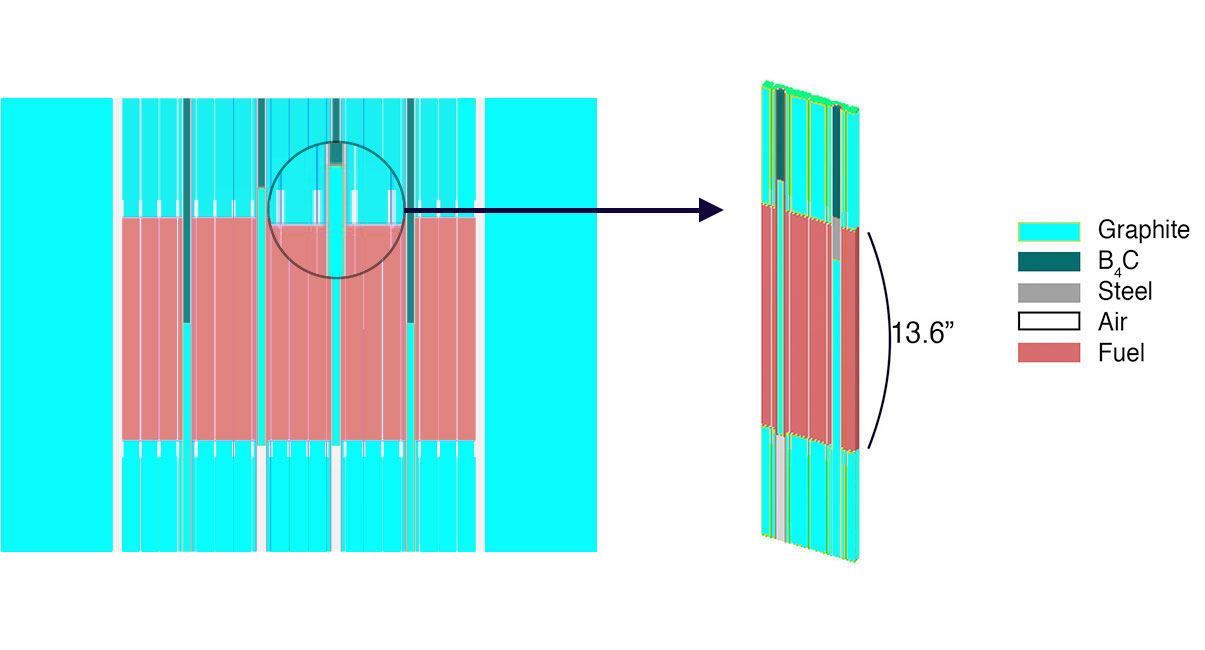
\includegraphics[width=14cm]{figures/big_to_small}
    \caption{The full TREAT core is given.  A control rod is shown larger to highlight the detail in the model.}
    \label{fig:treat3d}
\end{figure}

KENO writes out this tally style "mesh" in a proprietary file type with the extension .3dmap that may be read by several SCALE applications.  There are tools within SCALE to convert these file types to more generic ones such as VTK and SILO.  The VTK format, supported by VisIt, seemed the most appropriate as it appeared MOOSE could read those formats.  Upon further inspection this is not entirely true. MOOSE is only able to read unstructured XML based VTK files.  This is a newer format used by VisIt and supported by LibMesh.  So the simple conversion utility already available in SCALE was not useful as it was only able to convert from .3dMap to rectilinear VTK format.  In principle it would be possible to modify MOOSE to read these formats but would require significant changes according to the MOOSE team.  

The next thought was to convert from VTK rectilinear to VTK-XML unstructured.  It was possible to convert to XML with a GUI tool in VisIt but it remained a structured mesh.  With no way to map this KENO information into MOOSE the VTK XML was converted to .XYZ format.  This was read into MOOSE and it captured the nodal points correctly but all of the associated information about the fission density was lost. Directly converting the KENO mesh for MOOSE appears to require significant manipulation of both codes.

One more approach was attempted. That was incorporating the Exodus II API to construct a mesh directly from the KENO data.  Exodus is the preferred format in MOOSE.  The API allows for creation of exodus meshes fairly simply.  The difficulty came in the format KENO stored everything made the mapping between nodal points confusing and difficult to come up with a scheme that would work in general.  
Below highlights the conversion methods attempted.

$3dMap \rightarrow VTK (rectilinear) \rightarrow VTK-XML \rightarrow MOOSE$

$3dMap \rightarrow VTK (rectilinear) \rightarrow VTK-XML \rightarrow XYZ \rightarrow MOOSE$

$3dMap \rightarrow VTK (rectilinear) \rightarrow Exodus II\rightarrow MOOSE$

$3dMap \rightarrow Exodus II \rightarrow MOOSE$

Instead of converting the mesh into a format the MOOSE can already read it seemed reasonable to construct a mesh in MOOSE and map values onto it that approximately represents the geometry in KENO.  This seemed simpler as one can query mesh points in MOOSE and add values to it on the fly.  Instead of utilizing the .3dmap based mesh, the problem was discretized based on each fuel element of TREAT.  Note, this method is not robust and generally would only work for simple heat-up problems like in TREAT transients.  The fission density per unit was already given in KENO without additional tallies.  Our model of TREAT is organized into units of fuel elements positioned based on its location within a 2D array. See Figure \ref{fig:treat2d} below.  A unique unit may be constructed so the fission density is not averaged over similar repeated units.  Since the units were arranged into an array it is relatively simple to create the geometry in 2D and capture the radial fission or flux distribution.  Furthermore additional discretization may not have been useful due to the method our model was created and how the cross sections are generated.  Each fuel element unit has several materials/mixtures in it that are used to create multi-group cross sections. These materials may be re-used and therefor the cross section values re-used, even in different parts of the core at possibly different temperatures.  Updating the cross sections to new temperatures means assigning unique materials a new temperature and having that material correspond to a unique unit.  

A pseudo-mesh was created with a python script based on the location of each fuel element in two dimensions containing the corresponding fission density, temperature.  The progression from the KENO geometry to the mesh in MOOSE is shown in Figure \ref{fig:treat2d}.  A series of python scripts parse the KENO outputs to gather the fission density, create an (x,y) location for the center of each fuel element, and calculate the power density. It should be noted that KENO automatically provides the fission density in units of $fissions/cm^3$ and normalized per source neutron. The power density is calculated simply by multiplying the fission density by the average release per energy for U-235 and normalizing to the initial power.  In reality this energy/fission value is more complicated to calculate but for an initial test the simpler option was chosen. 

%\begin{figure}
%\centering
%\begin{minipage}{.5\textwidth}
%    \centering
%    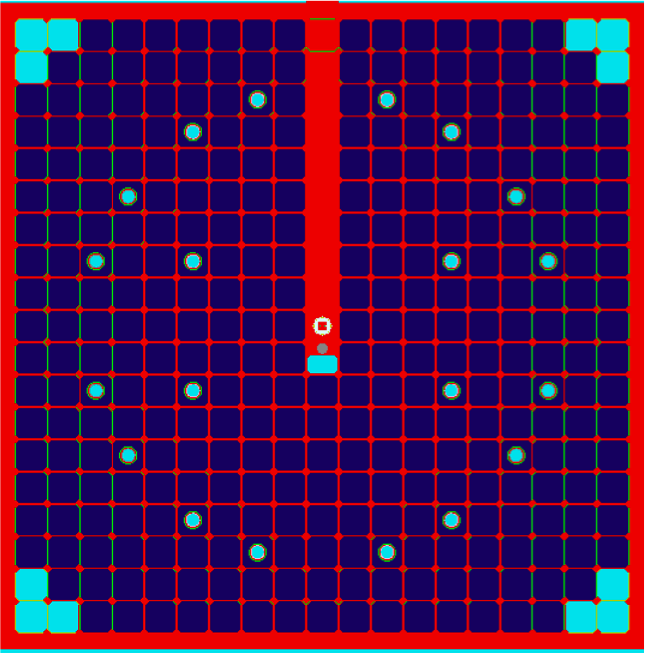
\includegraphics[width=6cm]{figures/treat_top_view.png}
%    \caption{Overview of TREAT model in two dimensions.}
%    \label{fig:treat2d}
%\end{minipage}%
%\begin{minipage}{.5\textwidth}
%  \centering
%  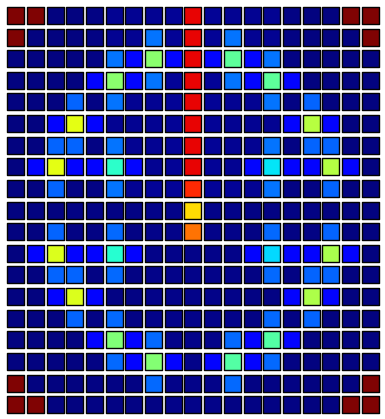
\includegraphics[width=6cm]{figures/simple-treat.png}
%  \caption{TREAT representation when mapping to MOOSE mesh.}
%  \label{fig:simpletreat}
%\end{minipage}
%\end{figure}

\begin{figure}
    \centering
    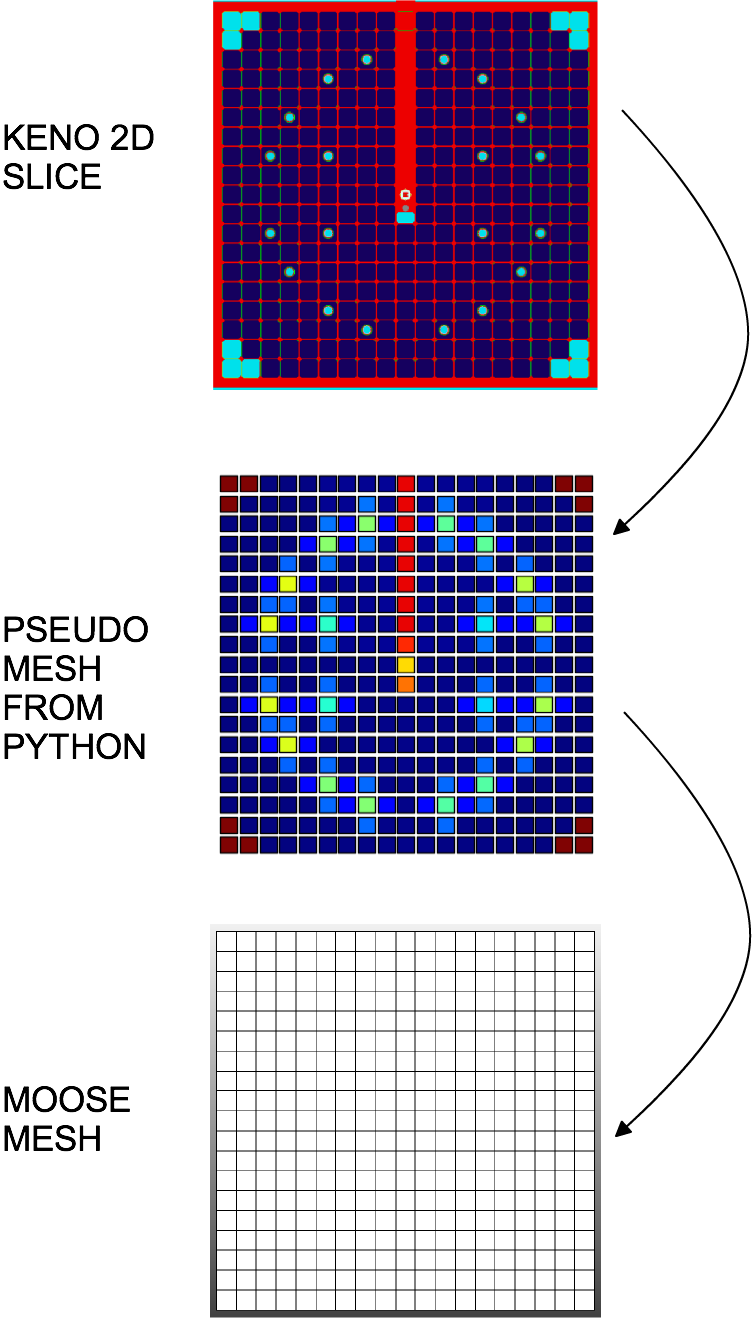
\includegraphics[width=6.5cm]{figures/progression-mesh.png}
    \caption{Progression of meshes as the information is mapped from KENO to MOOSE.}
    \label{fig:treat2d}
\end{figure}

	On the MOOSE side the goal is to solve the heat conduction problem with the power density as the heat source. A heat conduction module is already available within MOOSE.  This was modified slightly to read in the text file produced from the KENO data and assign a different thermal conductivity value and power density at each quadrature point.  The mesh generated in MOOSE is created \emph{a priori} to have approximately the same dimensions in 2D as the TREAT problem.  The KENO data was really providing values on nodal points but the values needed to be assigned on quadrature points, which are slightly offset from the nodal points.  This was achieved by simply determining the absolutely closest point from the KENO data to the corresponding quadrature point. 
	
\begin{figure}[h]
    \centering
    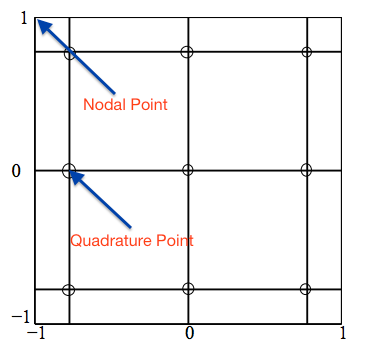
\includegraphics[width=8cm]{figures/nodalvsquad.png}
    \caption{Difference in nodal and quadrature mesh points}
    \label{fig:nodalquad}
\end{figure}

On the MOOSE side the stationary heat conduction equation is solved as described in the following:

\begin{equation}
    -\nabla \cdot k\nabla T - Q = 0
\end{equation}
where $k$ is the thermal conductivity in units of $[\frac{W}{cm K}]$  and $Q$ the power density in units of $[\frac{W}{cm^3}]$. The power density was calculated by multiplying the fission density from KENO by a $\kappa$ value of $3.11 \times 10^{-11} W/fission$. For fuel elements historical TREAT data is used for the thermal conductivity during heat-up (a different expression provides the thermal conductivity as the core cools).  This of course depends on temperature so the following expression is evaluated at the given temperature.

\begin{equation}
    k(T) = 5.08449 \times 10^{-8} * T^2 - 1.942915 \times 10^{-4} * T + 2.816049 \times 10^{-1}
    \label{cond}
\end{equation}

It should be noted that Equation \ref{cond} is only valid for temperatures between $250K$ and $1400K$.
At the time of writing the calculation runs and provides an answer.  The answers given appear unreasonable unfortunately when running it with the TREAT problem, as seen in Figure \ref{fig:moose-mesh}.  Given the time constraints it was not possible to evaluate the TREAT problem in greater detail.  Typically the results were too small or too large than would be expected.  A normalization to the thermal power is necessary when calculating the power density.  Several variations were attempted but changing this gave un-physical answers.  By unphysical, either temperature distributions were on the order of $10-8$ or $10^4$ on the Kelvin scale, again visible in Figure \ref{fig:moose-mesh}.  For this problem Dirichlet boundary conditions with $T=0$ were used.  The initial conditions were a constant $300K$ throughout.  

\begin{figure}[h]
    \centering
    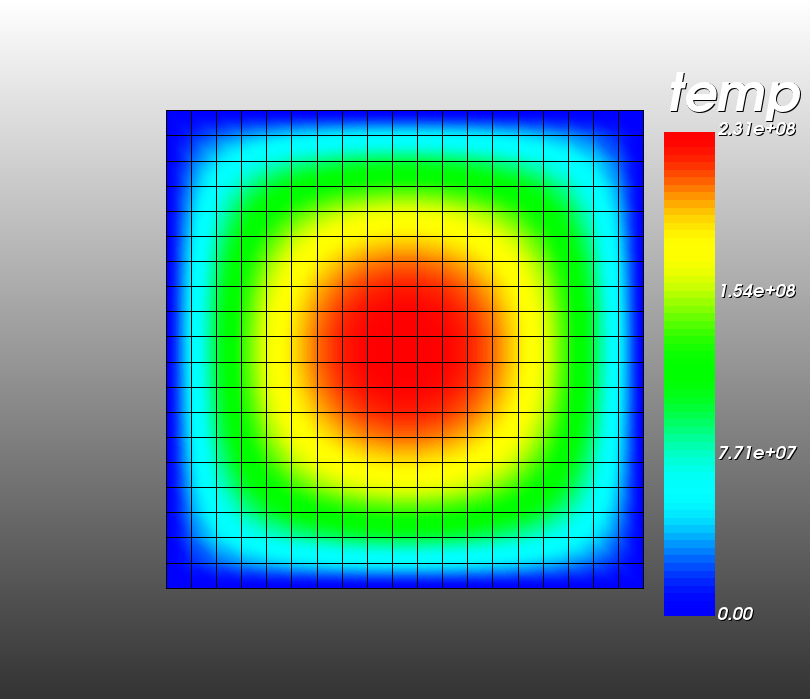
\includegraphics[width=8cm]{figures/large-with-mesh-temp.png}
    \caption{Initial result when solving the heat conduction equation on the MOOSE mesh.}
    \label{fig:moose-mesh}
\end{figure}

Despite the results of this effort not yielding anything concrete it still shows the proof of concept.  That KENO information may be mapped to MOOSE, albeit with some approximation.  The scripts and methods developed have been implemented to be automated once each component is verified to produce reasonable answers.  A diagram describing the ideal calculation flow is given in Figure \ref{fig:flow}.

\begin{figure}[h]
    \centering
    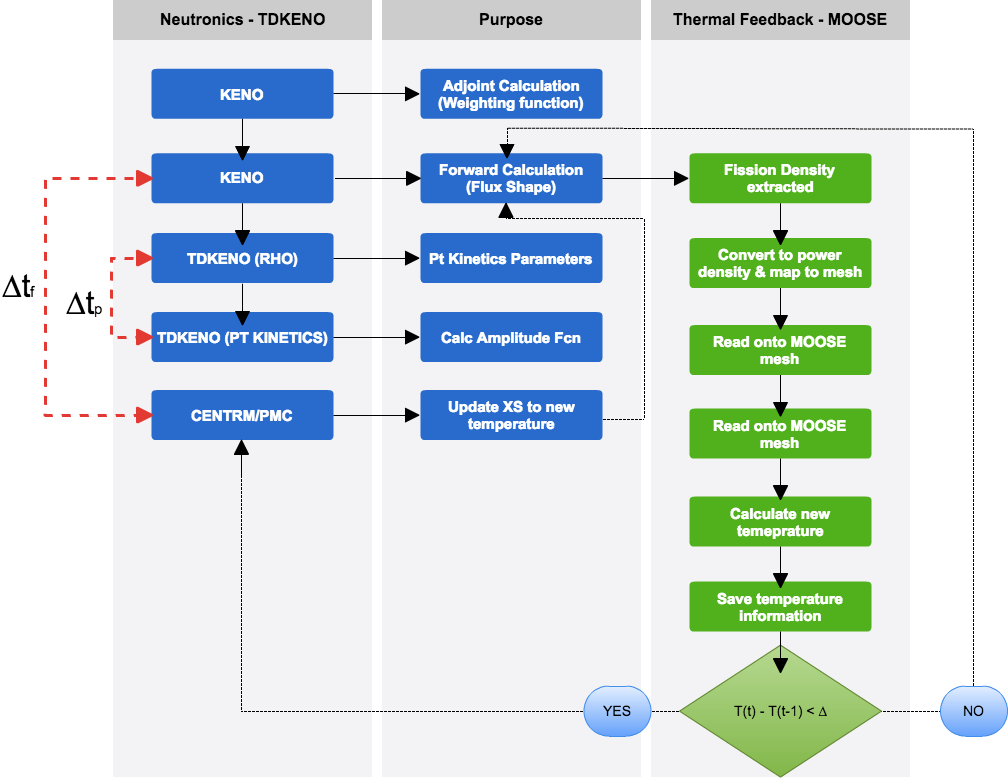
\includegraphics[width=16cm]{figures/flowcharttdk.png}
    \caption{Proposed flow chart for the coupling of TDKENO to MOOSE.}
    \label{fig:flow}
\end{figure}

\subsection{Adiabatic Heat Up Model}

In an effort to accomplish some kind of feedback a simple adiabatic heat-up model was quickly attempted.  This calculation may all be done within TDKENO, requiring no coupling to MOOSE.  With the rapid transients the heat may all be thought to be deposited locally in fuel elements and without significant interaction between elements.  Making this assumption the change in temperature from the fissions generated within a fuel element may be calculated with the following equation.

\begin{equation}
    \frac{dT(r,t)}{dt} = \epsilon \kappa \Sigma_f(T(r),t) \Psi(T(r),t) N
    \label{eq:adiabatic}
\end{equation}

In equation \ref{eq:adiabatic} $\epsilon$ is defined as $\epsilon = \frac{1}{\rho C_p}$ with $\rho$ as the density and $C_p$ as the heat capacity, $\kappa$ is the energy per fission, $\Sigma_f$ is the total fission cross section, $\Psi$ is the total angular flux, and $N$ is a normalization factor. For the heat capacity historical data is used for the TREAT problem.  Again this quantity is temperature dependent, so the following expression is evaluated before calculation.

\begin{equation}
    C_p(T) = -5.821 \times 10^{-10}*T^3 - 4.3694\times 10^{-7}*T^2 + 2.8369\times 10^{-3}*T - 1.009\times 10^{-2}
\end{equation}
This expression is valid from $273K$ to $810K$. The density value too is chosen from historical data, representing the total fuel element.   The values range from $1.71 g/cm^3$ $1.76g/cm^3$ depending on the concentration of uranium within graphite. 

In TDKENO this expression was found for each region in  geometry.  In KENO units are sub-divided into several regions. For instance a user can specify several axial regions per fuel element and this number can be varied with input generator made for TREAT simulations.  

The derivative in \label{adiabatic} was found with the backwards Euler method. The change in the temperature is added to a starting temperature of $300K$.  After each iteration the change in temperature for each region is found and added to the previous temperature. The temperatures are updated after each flux shape. The normalization factor ($N$) is based on the initial power of the system and is found by multiplying the fissionable volume by the power in and dividing that by the energy per fission. 

Once again there was not enough time to perform a thorough analysis but the temperatures found either increased by a few degrees or several thousand degrees.  This implementation is done on the scale of the flux shape.  For the benchmark problem 14-A2 in \cite{Bentley} the temperatures were calculated on the scale of the point kinetics solves.  The method differed slightly in that the fission cross sections were broadened within TDKENO and prepared for the next iteration.  This problem is simple with only 2 energy groups thus making the broadening relatively simple.  The approach implemented for the TREAT problem found the temperatures on the flux shape time scale because the cross sections could be evaluated by CENTRM/PMC.  Doing this method on the scale of the point kinetics would be too computationally expensive as CENTRM/PMC takes several minutes to run. The point kinetics calculations are solved hundreds of times between flux shapes.  Simpler methods may be implemented with TDKENO to broaden the cross sections but was not investigated thoroughly at this time.  Doing so may allow for coupling on the point kinetics time scale.   There is still work that needs to be done to get this method working.  For the TREAT specific problem feedback such as this will work for many of the transients. Future work should entail making this thermal feedback problem generalizable to problems beyond TREAT. 

\section{Cross-Section Processing}
No matter the method of coupling cross sections must be updated to the new temperature. Several approaches are possible with KENO at the time of writing.

1)	Updating the cross sections by creating a new set each time with the CENTRM/PMC utility within SCALE. Because CENTRM/PMC calculates a problem-dependent flux profile, it provides a rigorous cross-section treatment that explicitly handles effects from overlapping resonances, fissile material in the fuel and surrounding moderator, anisotropic scattering, and inelastic level scattering \cite{bowman2007overview}.  Basically, once MOOSE has calculated a new temperature for each fuel element this information is mapped back to the KENO input file.  Each units mixture has a new temperature.  The multi-group  cross sections are generated from these mixtures.  This input file is then processed with CENTRM/PMC to create unit dependent cross sections  based on the new temperature.  In most cases the unit will correspond to a unique fuel element. The cross section is then saved and placed in the TDKENO working directory.  The cross section creation time takes several minutes typically and adds another portion of the code to be externally coupled.  

2)  Instead of calculating the cross sections for each update, several cross sections for the same geometry may be made available before hand and interpolated within TDKENO to get as close to the new temperature as possible.  This requires knowing the range of temperatures the problem will be at.  For TREAT and many problems this is the case.  The approach still is not as robust as the first and likely not as accurate.

Briefly other codes methods will be summarized.  Other coupled codes rely on code-specific features to handle the temperature distribution and cross section creation.  For instance Serpent allows the cross sections to be updated on the fly with the Target Motion Sampling (TMS) temperature treatment \cite{viitanen2012explicit}. Additionally, Serpent may model a continuously varying density distribution \cite{leppanen2013modeling}.  The variation of density may be important in future problems so it is important to keep in mind.

OpenMC and MOOSE have been coupled as well.  The cross section updates are performed with an on-the-fly windowed multi-pole method for cross section Doppler broadening \cite{josey2016windowed}. This avoids interpolation of pre-generated cross sections or  weighting factors.  

Methods in OpenMC and Serpent are indeed  useful but may not be feasible options as TDKENO  currently relies  on KENO for the flux shape.  Each of these cross section processing methods relies on intricate processes ingrained in each respective code.  Mimicking such approaches would require significant modifications to KENO.  

%The MC21 Monte Carlo code implemented a clever "source" and "sink" approach where the user dictates %how the heat flows in the problem on top of the existing CSG geometry %\cite{griesheimer2008integrated}.  This requires lot of user pre-processing but requires no meshes %or discritizing the geometry beyond what is already defined.     


\section{Future Work}
All of the pieces are near  completion for a rudimentary coupling of TDKENO and MOOSE.  Given the time constraints it was not possible to complete a robust coupling between TDKENO and MOOSE.  There are several different options that may be pursued in the future to develop a code that simulates transients with accurate thermal feedback. Several will be outlined below. 

\subsection{Build TDKENO as a MOOSE App Explicitly}  
A natural extension of the summer work would be to build TDKENO under the MOOSE framework.  This would require a robust 3D mapping strategy from CSG geometry to meshes MOOSE understands.  Presumably as MOOSE evolves it will read additional mesh types and this may become easier.  Thus far it has proved challenging but it is not out of the scope of possibilities.   
There are significant disadvantages to this approach.

\begin{itemize}
    \item May have to build some SCALE based programs within MOOSE. Not a requirement but would make the coupling a bit "cleaner".  It is difficult as it is to build the latest version of SCALE (6.2) with the build system created at ORNL. One way around this is to build the KENO/CENTRM executable separately and only call them when needed.  The "TDKENO" portion, basically the point kinetics solver/flux modifier, would be built under MOOSE.
    \item Mapping from a CSG geometry to MOOSE type meshes is non-trivial.  A large point of using Monte Carlo is to get around the mesh creation portion of a simulation. Looking through the literature there are almost no coupled codes with KENO because of challenges like this.   
\end{itemize}

Conversely, there are several advantages to this method.
\begin{itemize}
    \item The internal coupling makes the code easier to adapt and improve. 
    \item As development progresses the solves on the MOOSE side may be made more complex to understand other phenomenon. For instance thermal expansion may be incorporated.  
    \item TDKENO would be able to compare with other codes that have adopted the MOOSE framework.  Comparisons are more meaningful if the codes are configured similarly. 
\end{itemize}

\subsection{Modify TDKENO to utilize a different Monte Carlo solver}
	In its current implementation TDKENO  calls upon a modified version of KENO to perform the flux shape.  The behavior is akin to an externally coupled code, with "TDKENO" driving the time dependence and calling KENO when it needs the flux shape. Presumably other codes could accomplish the same task.  One difficulty in choosing a code is many of the newer codes do not have the ability to perform an adjoint Monte Carlo calculation. In the  formulation of the governing TDKENO equations an adjoint calculation is performed and used as a weighting factor throughout.  Nevertheless there may be possibilities to modify the governing equations to get around this. For instance in Serpent it is not possible to perform an explicit adjoint calculation but one can weight calculations with the adjoint by using the iterated fission probability and keeping track of the progeny of neutrons in the forward simulation.  The goal of implementing a different code for the flux shape would be to implement one with a multi-physics framework already established.  A second, possibly over ambitious goal is to adopt a new flux shape solver and implement it in continuous energy.  Right now the formulation in TDKENO requires the flux shape be solved in multi-group, typically 238 groups.  Continuous energy calculation of the flux shape would provide greater rigor in IQS.  
	
	There are obviously several trade-offs in fundamentally modifying TDKENO that can be summarized in the following bullet points.
	
	Some disadvantages.
	\begin{itemize}
	\item These newer codes are not as mature and do not all possess the same features as KENO.  For instance in the calculation of the adjoint. Additionally, the cross section processing for creation of multi-group is excellent in SCALE and well tested (this could be side stepped by implementing a continuous energy calculation).
	\item This would require significant rewriting of TDKENO.  
	\item May have to re-derive some of the governing equations to account for differences in the flux shape solvers ability.
	\item Implementing continuous energy would in itself be a large undertaking.  Almost definitely would require re-defining the IQS problem statement.
	 Some advantages of this approach are enticing.
	 \end{itemize}
	\begin{itemize}
	\item Adopting a code that can easily interface with other physics codes makes coupling easier and more robust.  
	\item More "modern" codes are in theory easier to craft for unique purposes such as IQS.  Modern coding practices are useful for testing new features and building across different platforms.  Currently, using KENO from SCALE 6.2 it has been difficult to build on many computers.
	\item Creating an IQS method utilizing continuous energy would make it a state of the art transient solver.
	\end{itemize}	
	  
\subsection{Continue using KENO but introduce Functional Expansion Tallies}
To get around complex mapping of geometries and discretization of the Monte Carlo geometry the Functional Expansion Tally(FET) method may be introduced in KENO.  Here values of interest may be tallied and the distribution represented by well known polynomials.  This has been the method introduced in OpenMC with good results and recently in Serpent 2 with encouraging results.  More than 10 years ago FETs were implemented in MCNP4  but with simpler polynomials \cite{griesheimer2004two}. This would indicate its possible to do in KENO as well due to MCNP's similarities to KENO. Both OpenMC and Serpent recreated radial distributions of power and temperature with Zernike polynomials  for cylindrical fuel elements.  Several example Zernike polynomials are in Figure \ref{fig:zernike}. In the axial direction, Legendre polynomials are used. 

\begin{figure}
    \centering
    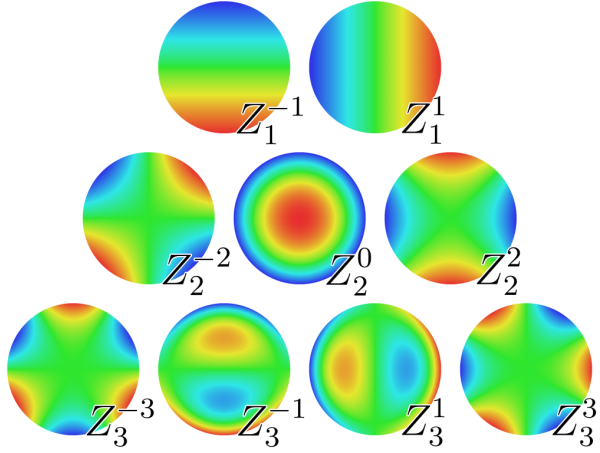
\includegraphics[width=10cm]{figures/zernike-circle.png}
    \caption{Several examples of Zernike functions in an octagon \cite{ferreira2015orthogonal}}.
    \label{fig:zernike}
\end{figure}

Utilizing the traditional Zernike Polynomials works well on cylindrical fuel elements as they are only guaranteed to be orthogonal on circular domains.  However, for  TREAT simulations many of the fuel elements are not circular but are octagon like.  Using Zernike polynomials as implemented in OpenMC and Serpent may not represent the distributions exactly.  Fortunately a recent paper outlines a generalized method for mapping between circular to greater than 3 sided polygons \cite{ferreira2015orthogonal}.  In this paper the authors outline one case where they derive Zernike polynomials that are orthogonal on an octagon, several of these are provided in Figure \ref{fig:oct-fet}. For the TREAT problem the 8-sided case would need to be modified for sides that are not all the same but with every other side the equal.  It seems in principle possible.  Zernike polynomials for both circular and octagonal domains should be similar and would be implemented at the same time.  The user would then be able to choose which to use based on the governing problem.  
\begin{figure}
    \centering
    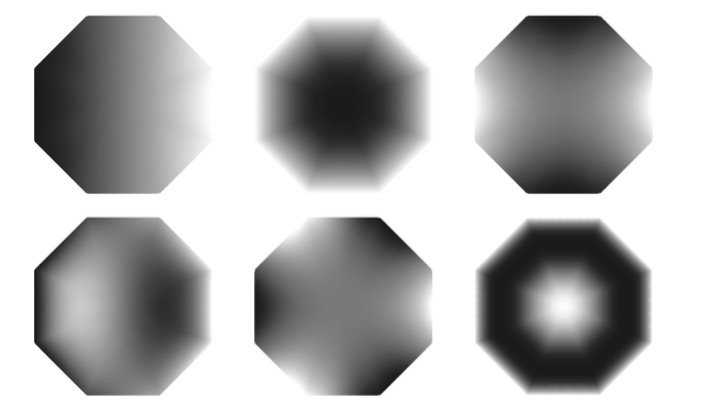
\includegraphics[width=8cm]{figures/octogon-FET.png}
    \caption{Several examples of Zernike functions in an octagon \cite{ferreira2015orthogonal}}.
    \label{fig:oct-fet}
\end{figure}
 
Some disadvantages to this approach are highlighted below.
	\begin{itemize}
	\item Further developing capabilities in KENO makes it difficult to adopt a new code in the future.
	\item Modifying KENO source code may be more difficult than Serpent or OpenMC.
	\item FETs are still untested in many applications.  Many of the problems using them have been academic type in two dimensions or three dimensions in single pins.  These challenges may be compounded looking at FETs on polygonal domains.  These type of modified Zernike polynomials  appears to not have been implemented before in nuclear engineering applications. 
	\item This would force the coupling to only be done on the largest time scale in IQS.  If the temperature distribution is thought to change on a smaller scale this would cause complications.  Some early IQS papers suggest the feedback needs to be done in-between flux shape calculations. 
	\item This methodology it somewhat limited to analysis of fuel elements with specific geometry types.  For instance pebble bed reactors would be incompatible with this implementation.
	\end{itemize}

Significant advantages are gained from this approach:
	\begin{itemize}
	\item As mentioned continuous temperature and power distributions are constructed in great detail without complications of mesh mapping or discretizing the geometry.
	\item Only passing coefficients makes for minimal memory usage.
	\item Since similar methods are already implemented in  the OpenMC/MOOSE integration it would make the coupling between TDKENO and MOOSE easier. 
	\item The TDKENO source code would not require significant modifications. 
	\item Implementing FETs in KENO would in itself be useful beyond TREAT simulations.  Time independent problems may benefit from such methods as well. 
	\end{itemize}


\subsection{Solving the heat conduction problem via Monte Carlo techniques}

The last suggestion for a future coupling implementation  fundamentally differs from the previous 3.  Instead of solving the heat conduction  with finite element analysis the problem may be solved via Monte Carlo.  This idea has been looked at several times in the past 50 years\cite{fraley1980monte, hoffman1976monte, haji1967solution}.  Early studies showed the computational cost prohibitively  expensive but promising due to the ability to handle complex geometries.  Since the diffusion approximation in transport theory is mathematically equivalent to the heat conduction problem there are many analogous methods. Recent work has been done in Korea and a code has been developed to solve the heat conduction problem via Monte Carlo with MCNP as the geometric engine  \cite{song2007improved}.  The motivation for their study was investigation of the temperature variation in pebble bed reactors.  Reactors of this type would be difficult to simulate with finite element methods due to the large number of small fuel particles.  The lack of mesh makes the coupling straightforward and obviously requires no discretization. Problems involving time dependence are largely unstudied with this method.  Implementing thermal feedback in this manner would be a novel concept in transient analysis.

Obviously there are disadvantages with the Monte Carlo approach including:
	\begin{itemize}
	\item Computational time is almost guaranteed to be larger than comparable deterministic methods.  Though Monte Carlo techniques have become more palatable as access to large scale computers is a given in a major research center.
	\item Will  require significant programming from the ground up. 
	\item  This approach will be tied to a specific geometry definition introduced by the neutronics solver.  
	\item  There is no connection with a general solver such as MOOSE.  The physics that one would be able to study is limited.  Problems such as material movement would require additional efforts, unlike using a general solver like MOOSE, where in principal it is possible to couple with other physics built upon the framework.
	\item The temperature distributions would not be continuous in this method as Monte Carlo techniques average the integral over each respective region.
	\end{itemize}

The advantages of going to a code that mainly uses Monte Carlo has several advantages:
	\begin{itemize}
	\item The most obvious  of using Monte Carlo throughout is no loss of information going from CSG to mesh based geometries. 
	\item Makes this approach generalizable to geometries modeled with CSG. Problems beyond TREAT could make use of TDKENO.  
	\item Could explore developing this code for new architectures such as graphics processing units (GPUs).  The investigation of Monte Carlo problems on such accelerators is of great interest as  high performance computing is trending towards adopting this technology (e.g. Titan Super Computer at ORNL has over 18,000 GPUs). 
	\item Cross sections could be generated on the fly since the temperature information for each region would be ready and easily accessible.  This further simplified the coupling as cross sections processing is a somewhat tricky detail going between codes. 
	\end{itemize}

The flexibility this approach offers is enticing.  There is lots of opportunity for fundamental research to be done, particularly in the transient analysis setting.  Furthermore it provides an opportunity to write code for the next generation of computing architectures.  While there are implementation unknowns, the theoretical background for this problem is generally well understood. The transient analysis portion as mentioned is largely unstudied but is ripe for investigation.  TDKENO being a code already based on a Monte Carlo technique is an ideal candidate for such an investigation.


\section{Conclusions}

A preliminary attempt at coupling TDKENO and MOOSE has many of the components in place but  requires additional development to attain reasonable answers.  The methods looked at may not be robust enough for future problems.  There is a variety of coupling techniques that may be implemented in future iterations of TDKENO.  There are several trade offs to consider in development time and target application.  Some methods may be easier to implement but will not be useful on a broad class of problems.  Any of the methods outlined in the future work section will help TDKENO to become a tremendous utility for transient analysis. 

\section{Acknowledgments}
I would like to thank Leslie Kerby and Mark DeHart for their guidance on this work performed at the INL.  Additionally, I must thank my adviser Sedat Goluoglu for setting up this endeavor and responding to emails even when half way across the world.  
Finally, I must thank the INL for financial support for this work and on site resources.  The experience was invaluable and I feel I have learned a tremendous amount.

\bibliographystyle{unsrt}
\bibliography{bibliography}

\end{document}

